% template created by: Russell Haering. arr. Joseph Crop
\documentclass[12pt]{article}
\usepackage[hmargin=1in, vmargin=1in]{geometry}
\usepackage{fancyhdr}
\pagestyle{fancy}
\usepackage[hang,small]{caption}
\usepackage{lastpage}
\usepackage{graphicx}
\usepackage{verbatim}
\DeclareGraphicsExtensions{.jpg}
\usepackage{url}

\def\author{Jacques Uber and Kevin Ngo}
\def\title{ECE472 Lab2 Report}
\def\date{\today}

\fancyhf{} % clear all header and footer fields
\fancyhead[LO]{\author}
\fancyhead[RO]{\date}
% The weird spacing here is to get the spacing of \thepage to be right.
\fancyfoot[C]{\thepage\
                    / 7}

                    \setcounter{secnumdepth}{0}
                    \setlength{\parindent}{0pt}
                    \setlength{\parskip}{4mm}
                    \linespread{1.4}


\begin{document}
\fancyhf{} % clear all header and footer fields
\fancyhead[LO]{\author}
\fancyhead[RO]{\date}
\fancyhead[CO]{\title}



\section{Lab 2 Report}
    In this lab we implemented a 16 bit Carry Lookahead adder and compared it to a 16bit Ripple Carry adder.
\begin{enumerate}
    \item
        Here is a block diagram of the 16 bit Carry lookahead adder.

    \includegraphics[scale=0.55]{img/16bit_cla.png}


    \item
        Show the initial ripple adder working and it's wave form (Problem 8)

    \includegraphics[scale=0.55]{img/problem_8.png}

    \item Lab Code
    {\tiny
    \begin{verbatim}
/*
* Kevin Ngo and Jacques Uber
* 16 bit adder using 4 r-bit Carry-lookahead-adders
*/

module add16_LA(a, b, sum, cout);
    input [15:0] a, b;

    output cout;
    output [15:0] sum;

    wire [3:0] c; // LA module carries

    wire [3:0] super_p;
    wire [3:0] super_g;
    wire cin;
    assign cin = 0;
    assign cout = c[3];

    wire [1:0] p_g; // We don't care about these

    cla_4bit cla0(a[3:0], b[3:0], sum[3:0], cin, super_p[0], super_g[0]);
    cla_4bit cla1(a[7:4], b[7:4], sum[7:4], c[0],  super_p[1], super_g[1]);
    cla_4bit cla2(a[11:8], b[11:8], sum[11:8], c[1], super_p[2], super_g[2]);
    cla_4bit cla3(a[15:12], b[15:12], sum[15:12], c[2], super_p[3], super_g[3]);
    lookahead large_cla(super_p, super_g, c[3:0], cin, p_g[0], p_g[1]);
endmodule
/*
* Kevin Ngo and Jacques Uber
* A simple 4 bit adder
* Part 11 of the lab
*/

module cla_4bit(a, b, sum, cin, p0, g0);
    input [3:0] a, b;
    input cin;
    output [3:0] sum;
    output p0, g0;

    wire [3:0] la_p_out;
    wire [3:0] la_g_out;
    wire [3:0] c;


    fulladder_LA f0(a[0], b[0], cin, sum[0], la_p_out[0], la_g_out[0]);
    fulladder_LA f1(a[1], b[1], c[0], sum[1], la_p_out[1], la_g_out[1]);
    fulladder_LA f2(a[2], b[2], c[1], sum[2], la_p_out[2], la_g_out[2]);
    fulladder_LA f3(a[3], b[3], c[2], sum[3], la_p_out[3], la_g_out[3]);
    lookahead la0(la_p_out, la_g_out, c[3:0], cin, p0, g0);
endmodule
/*
* Kevin Ngo and Jacques Uber
* A full adder with lookahead
*/

module fulladder_LA(a, b, cin, sum, p, g);
    input a, b, cin;
    output sum, p, g;

    assign #2 sum = a ^ b ^ cin; // Worst case delay is 2
    assign #1 g = a & b; // Worst case delay is 1
    assign #1 p = a ^ b; // Worst case delay is 1
endmodule
/*
* Kevin Ngo and Jacques Uber
* A full adder
*/

module fulladder(a, b, cin, sum, cout);
    input a, b, cin;
    output sum, cout;

    // Problem 13 adds delay
    assign #2 sum = a ^ b ^ cin; // Worst case delay is 2
    assign #2 cout = a & b | a & cin | b & cin; // Worst case delay is 3
endmodule
/*
* Kevin Ngo and Jacques Uber
* carry-look-ahead module
* Input 4 pg (8 wires)
* Output 4 c (4 wires)
*/

module lookahead(p, g, c, cin, p0, g0);
    input [3:0] p, g;
    input cin;
    output [3:0] c;
    output p0, g0; // The Super P and G

    assign #2 c[0] = g[0] | p[0] & cin;
    assign #3 c[1] = g[1] | g[0] & p[1] | cin & p[0] & p[1];
    assign #4 c[2] = g[2] | g[1] & p[2] | g[0] & p[1] & p[2] | cin & p[0] & p[1] & p[2];
    assign #5 c[3] = g[3] | g[2] & p[3] | g[1] & p[2] & p[3] | g[0] & p[1] & p[2] & p[3] | cin & p[0] & p[1] & p[2] & p[3];

    assign #3 p0 = p[3] & p[2] & p[1] & p[0];
    assign #4 g0 = g[3] | p[3] & g[2] | p[3] & p[2] & g[1] | p[3] & p[2] & p[1] & g[0];
endmodule
/*
* Kevin Ngo and Jacques Uber
* Lab1 testbench
* We want to simulate both the ripple adder and the carry look ahead adder at the same time. This
* will allow us to see the wave forms in the same window and allow for easier analysis.
* Any thing that has 'LA' or 'la' is assumed to be part of the 'Look Ahead' adder.
*/

module proj2_testbench;

    reg clk; // Both LA and non-LA use the same clock

    wire [15:0] sum;
    wire cout;
    reg [15:0] A, B;


    // DUT = Device under test
    ripple_adder DUT(A, B, sum, cout);

    wire [15:0] sum_LA; // LA get's its own sum
    wire cout_LA; // LA get's it's own cout
    reg [15:0] A_la, B_la; // LA get's it's own inputs

    add16_LA lA(A_la, B_la, sum_LA, cout_LA);

    always
        #5 clk=~clk;

    initial begin
        clk = 1'b0;
        A = 8;
        B = 31;
        A_la = 8;
        B_la = 31;
    end

    always @(posedge clk)
    begin
        A = A + 1;
        //B = B + 0;
        A_la = A_la + 1;
        //B_la = B_la + 0;
    end
endmodule
/*
* Kevin Ngo and Jacques Uber
* A ripple carry adder with and without Lookahead
*/

module ripple_adder(a, b, sum, cout);

    input [15:0] a, b;
    output [15:0] sum;
    output cout;

    wire [15:0] c;
    assign c[0]=0;
    fulladder f0(a[0], b[0], c[0], sum[0], c[1]);
    fulladder f1(a[1], b[1], c[1], sum[1], c[2]);
    fulladder f2(a[2], b[2], c[2], sum[2], c[3]);
    fulladder f3(a[3], b[3], c[3], sum[3], c[4]);
    fulladder f4(a[4], b[4], c[4], sum[4], c[5]);
    fulladder f5(a[5], b[5], c[5], sum[5], c[6]);
    fulladder f6(a[6], b[6], c[6], sum[6], c[7]);
    fulladder f7(a[7], b[7], c[7], sum[7], c[8]);
    fulladder f8(a[8], b[8], c[8], sum[8], c[9]);
    fulladder f9(a[9], b[9], c[9], sum[9], c[10]);
    fulladder f10(a[10], b[10], c[10], sum[10], c[11]);
    fulladder f11(a[11], b[11], c[11], sum[11], c[12]);
    fulladder f12(a[12], b[12], c[12], sum[12], c[13]);
    fulladder f13(a[13], b[13], c[13], sum[13], c[14]);
    fulladder f14(a[14], b[14], c[14], sum[14], c[15]);
    fulladder f15(a[15], b[15], c[15], sum[15], cout);
endmodule

    \end{verbatim}
    }

    \item
    Print to pdf or take screenshots of the waveform timing diagrams that show delays for several input conditions including the worst case delay

    \subitem
    Some examples of adding arbitrary numbers being added (including delay).

    \includegraphics[scale=0.50]{img/correct_math.png}

    \subitem
    Wort Case Delay

    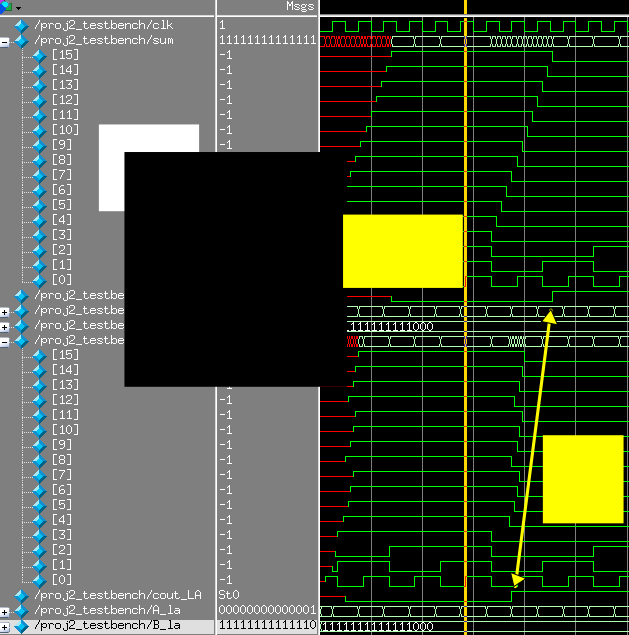
\includegraphics[scale=0.7]{img/worst_case_delay3.png}

    \item
    Finally, indicate your estimate of the amount of time you spent on this project, what you  felt  was  most  valuable  and  least  valuable  about  this  project,  and  any suggestions you might have for improving this project in the future.

    We spent close to 5 or 6 hours on this.
\end{enumerate}
\end{document}

